
\section{Continuous Integration Health}
\label{sec:ci}

The CI census reads the last workflow run per repository. Of 130 active repositories:
\begin{itemize}
\item \textbf{121} last-run \texttt{success};
\item \textbf{1} \texttt{action\_required} (a review-gated repository whose required check is a dead protection context --- an owner-action deadlock, documented, not bypassed);
\item \textbf{2} transient (\texttt{pending}/\texttt{in\_progress} at read time);
\item \textbf{6} \texttt{NO\_RUNS} (three repositories with no workflows by design --- a backup repository, a sandbox, and an acoustic research repository --- and three GHSA advisory placeholders).
\end{itemize}
The \texttt{action\_required} case deserves its own sentence: the repository's branch protection references a required check that no longer exists on any workflow path (a dead protection context), so every run ends awaiting an owner action that no automation may perform. The doctrine-correct treatment is exactly this paragraph --- a deadlock published in a census, not a protection gate quietly dropped to turn the census green. Zero repositories were disabled manually. Figure~\ref{fig:ci} shows the distribution. The single \texttt{action\_required} case is reported here precisely because the estate's doctrine forbids silently bypassing a protection gate to turn a red census green: the deadlock itself is the receipt.

\begin{figure}[htbp]
\centering
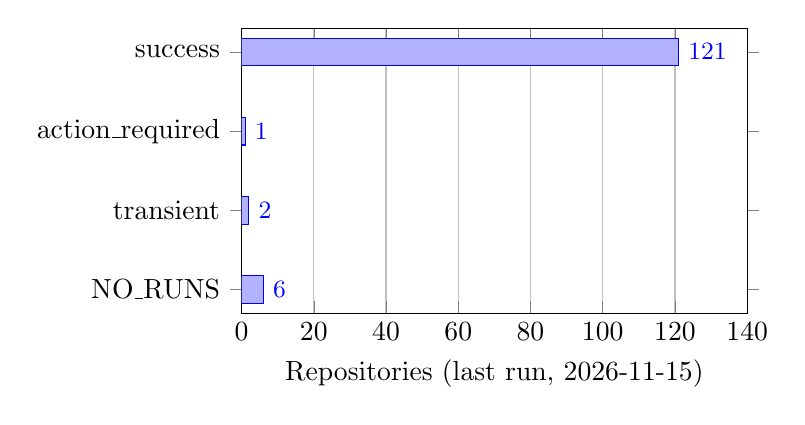
\begin{tikzpicture}
\begin{axis}[
  xbar, width=0.66\textwidth, height=5.2cm,
  symbolic y coords={NO\_RUNS, transient, action\_required, success},
  ytick=data, xmin=0, xmax=140,
  xlabel={Repositories (last run, 2026-11-15)},
  nodes near coords, every node near coord/.append style={font=\small},
  ymajorgrids=false, xmajorgrids=true,
]
\addplot coordinates {(121,success) (1,action\_required) (2,transient) (6,NO\_RUNS)};
\end{axis}
\end{tikzpicture}
\caption{CI health of the 130 active repositories. The action\_required deadlock is disclosed rather than bypassed.}
\label{fig:ci}
\end{figure}

\section{The Receipt Substrate}
\label{sec:substrate}

The estate's receipts live in versioned Hugging Face datasets, addressed by repository and commit. The largest receipt dataset, \texttt{SZLHOLDINGS/frontier-54-runs}, exposes more than one thousand files through the tree API (which caps at 1000 entries; the true count is at least the cap). Table~\ref{tab:namespaces} and Figure~\ref{fig:namespaces} give the namespace distribution at census time.

\begin{table}[htbp]
\centering
\small
\begin{tabular}{lr}
\toprule
\textbf{Namespace} & \textbf{Files} \\
\midrule
\texttt{mesh/} (GPU-worker run receipts) & 872 \\
\texttt{benchmark/} (evaluation batteries) & 67 \\
\texttt{collaboration/} (co-signed instruments) & 11 \\
\texttt{deploy/} & 10 \\
\texttt{doctrine/} & 7 \\
\texttt{receipts/} (dated sweep receipts) & 7 \\
\texttt{lean/} & 6 \\
\texttt{census/} & 5 \\
\texttt{competitive/}, \texttt{wheels/}, \texttt{data/}, \texttt{energy/} & 2 each \\
\texttt{tools/}, \texttt{officers/}, \texttt{monetization/}, \texttt{registry/}, \texttt{proving-ground/} & 1 each \\
\midrule
\textbf{Total (API-capped)} & \textbf{$\geq$1000} \\
\bottomrule
\end{tabular}
\caption{Namespace distribution of \texttt{frontier-54-runs} on 2026-11-15. The tree API returns at most 1000 entries; the mesh namespace dominates because every GPU worker checkpoint writes a receipt.}
\label{tab:namespaces}
\end{table}

\begin{figure}[htbp]
\centering
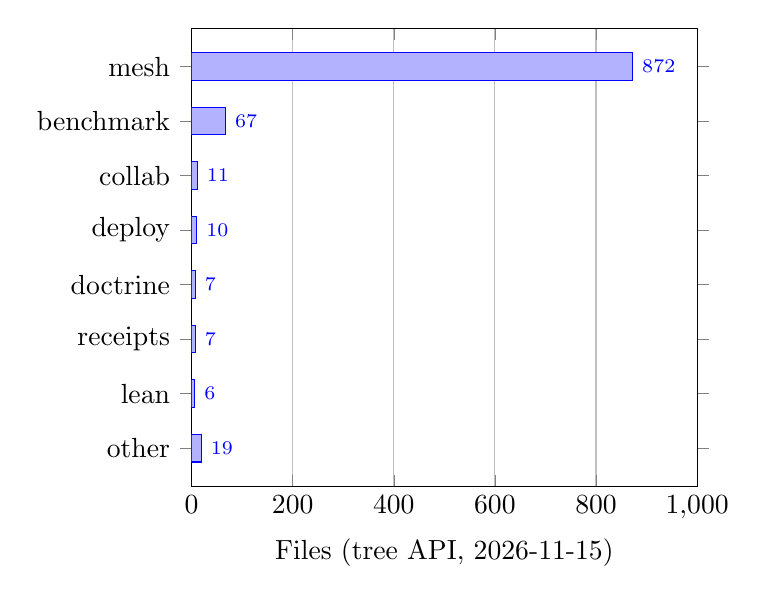
\begin{tikzpicture}
\begin{axis}[
  xbar, width=0.66\textwidth, height=7.4cm,
  symbolic y coords={other, lean, receipts, doctrine, deploy, collab, benchmark, mesh},
  ytick=data, xmin=0, xmax=1000,
  xlabel={Files (tree API, 2026-11-15)},
  nodes near coords, every node near coord/.append style={font=\scriptsize},
  xmajorgrids=true,
]
\addplot coordinates {(872,mesh) (67,benchmark) (11,collab) (10,deploy) (7,doctrine) (7,receipts) (6,lean) (19,other)};
\end{axis}
\end{tikzpicture}
\caption{Receipt distribution by namespace (\textquotedblleft other\textquotedblright{} aggregates the sub-10 namespaces). The mesh namespace's 872 receipts are per-worker-run records from the SaladCloud GPU lanes.}
\label{fig:namespaces}
\end{figure}

Eight Zenodo DOIs pin the preprint lineage (the umbrella record is \texttt{10.5281/zenodo.19944926}); the DOI registry lives in \texttt{szl-papers} and a consistency checker enforces that every README claiming a measured section carries a live deposit.

\section{Formal Verification: The Lean 4 Corpus}
\label{sec:lean}

The proof corpus \texttt{szl-holdings/lutar-lean} is a Lean~4/Mathlib project whose disclosure discipline separates three registries that are easy to conflate and fatal to conflate publicly:
\begin{enumerate}
\item the \textbf{locked-proven formula registry}, which moved from five to exactly eight entries (\texttt{locked\_count\_eight}, proved \texttt{by decide}), containing the focal governance invariants F1, F4, F7, F11, F12, F18, F19, F22;
\item the \textbf{canonical declaration baseline} 749/14/163 (theorems/definitions/instances) frozen at the earlier doctrine commit \texttt{c7c0ba17} --- a distinct object from the proof snapshot;
\item the \textbf{proof snapshot} \texttt{5cfaf9a3} at which the three newest invariants (F4 acyclicity preserved under append, F7 FIFO batch drain with positional equality witness, F22 strictly monotone emit log) are kernel-checked and non-vacuous.
\end{enumerate}

The corpus ledger at the audited commit records 12 declarations in the audit-workflow set, 5 in the pipeline set, and 8 in the locked set (Figure~\ref{fig:ledger}); per-classifier witness-class counting records $\varnothing$=7, $\{P\}$=4, $\{P,Q\}$=1, $\{P,C,Q\}$=13 (Figure~\ref{fig:verdict}), with final verdicts 3 confirmed, 2 conditional, 2 refined, 1 held.

\begin{figure}[htbp]
\centering
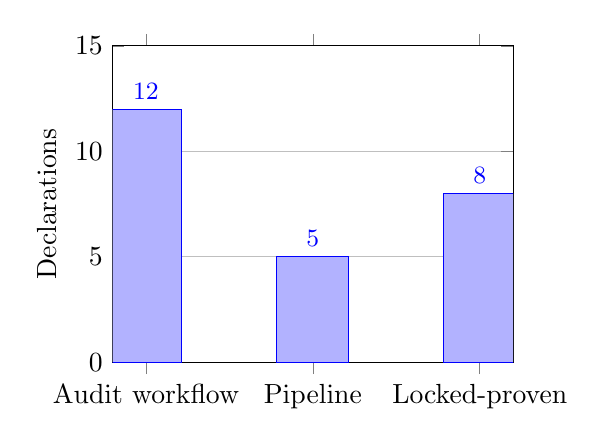
\begin{tikzpicture}
\begin{axis}[
  ybar, bar width=26pt,
  width=0.55\textwidth, height=5.6cm,
  symbolic x coords={Audit workflow, Pipeline, Locked-proven},
  xtick=data, ymin=0, ymax=15,
  ylabel={Declarations},
  nodes near coords, every node near coord/.append style={font=\small},
  ymajorgrids=true,
]
\addplot coordinates {(Audit workflow,12) (Pipeline,5) (Locked-proven,8)};
\end{axis}
\end{tikzpicture}
\caption{Declaration ledger by registry at the audited corpus commit. The locked-proven set is exactly eight; the count is machine-checked (\texttt{locked\_count\_eight}, \texttt{by decide}).}
\label{fig:ledger}
\end{figure}

\begin{figure}[htbp]
\centering
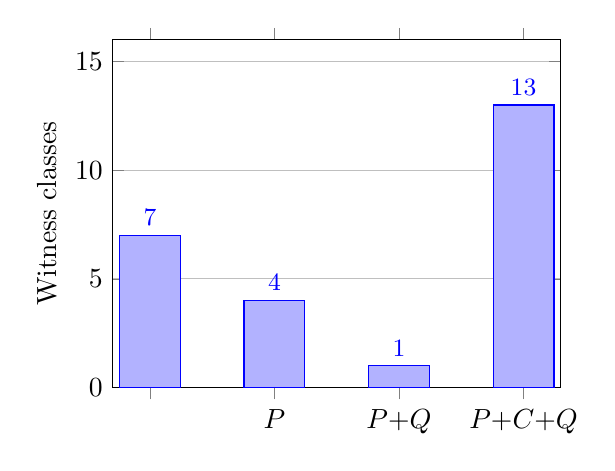
\begin{tikzpicture}
\begin{axis}[
  ybar, bar width=22pt,
  width=0.6\textwidth, height=6.0cm,
  symbolic x coords={none, P, PQ, PCQ},
  xtick=data, ymin=0, ymax=16,
  xticklabels={$\varnothing$, $P$, $P{+}Q$, $P{+}C{+}Q$},
  ylabel={Witness classes},
  nodes near coords, every node near coord/.append style={font=\small},
  ymajorgrids=true,
]
\addplot coordinates {(none,7) (P,4) (PQ,1) (PCQ,13)};
\end{axis}
\end{tikzpicture}
\caption{Witness-class distribution over the audited declaration set ($P$ = proof term, $Q$ = qualifier, $C$ = constructor evidence). The mass in $\{P,C,Q\}$ reflects the non-vacuity audit: a bare proof term without constructor evidence is not admitted to the registry.}
\label{fig:verdict}
\end{figure}
